% !TEX root = ../main.tex

\section{Background}
\label{section:background}

In this section, we use a traditional statistical framework as a guideline for multilabel classificaton methods~\citep{tukey}. We distinguish the desired theoretical statistic (the \textbf{estimand}), its functional form (the \textbf{estimator}) and its approximation (the \textbf{estimate}); the latter estimates can be benchmarked with \textbf{metrics}. We show how multilabel reductions tend to reformulate the estimand and treat labels independently (i.e. change\daan{or make addtional?} the assumptions about the data). However, with an appropriate\daan{well-chosen? well-designed? properly formulated?} estimator, it is possible to directly model the estimand. Our proposed loss function, \textbf{multilabel blend}\daan{introducing a new name here}, accommodates for the true estimand. This section ends with a mention of the multiclass setting, where the estimand-estiomator-estimate triad is more straightforward.\daan{Last sentence seems out of line here.} \daan{If multiclass is so straightforward, could we use it here to illustrate the background before we cover multilabel?}

We define a learning algorithm that maps inputs to outputs given a set of hyperparameters \(\mathcal{F}(\cdot ; \Theta): \mathcal{X} \rightarrow \mathcal{Y}\). \todo{$\mathcal{F}$ is the estimator that produces   the estimate $\mathcal{Y}$.}

\subsection{Estimand: definition of the risk}
\label{section:background:estimand}

We consider a classification setting with $C$ classes and distinguish between two scenarios: the \emph{multilabel} and the \emph{multiclass} scenario. 
In the multilabel scenario, a single example can be assigned more than one class label (e.g., movie genres). 
In the multiclass scenario, a single example has only one class label \todo{?stemming from an example?} (e.g., classification of an animal on a picture). 
%Multiclass classification deserves a mention towards the end, as it illustrates a straightforward relationship between estimand-estimator-estimate. 
We focus on the multilabel scenario; its risk formulation can be written as in ~\citep{multilabelReduction}:
%
\begin{equation}
R_{\mathrm{ML}}(\mathcal{F}) = \mathbb{E}_{(x, y)}\left[\ell_{\mathrm{ML}}(y, \mathcal{F}(x))\right].
\end{equation}
%
We define \emph{risk} as the estimand: the theoretical statistic. For example, there is a finite number of animals ($y_{corn}$) that eat corn ($x_{corn}$), assuming animals belong to a finite set of living beings. The theoretical risk (estimand) defines that exact deterministic quantity $y_{corn}$. 
\daan{Wait, x is not features?}
In practice, statistical models do output probabilities via an estimator and its estimate (also called propensities or suitabilities~\citep{multilabelReduction}). The solution to that stochastic-deterministic incompatibility is either to convert the estimator to a deterministic measure via decision thresholds (traditional cross-entropy loss), or to reformulate the estimand as a stochastic measure (our multilabel blend proposal).

\subsection{Estimator: the functional form of the risk}
\label{section:background:estimator}

The estimator $f \in \mathcal{F}$ is any minimizer of the risk $R_{ML}$. 

\begin{proposition}
  The multilabel estimator of $y_i$ is dependent on the input and other labels for that example,
%
\begin{equation}
  \hat{y}_i = \mathcal{F}(x, y_1, \ldots, y_C) = P(y_i = 1 | x, y_1, \ldots, y_C) \, \forall y_j \, not \, in \, y_i
\end{equation}
\label{eq:estimand}
\end{proposition}
%
Predicting multiple labels per example comes with the assumption that labels are non-mutually exclusive. By proposing this general formulation, we entrench that characteristic in the estimator. Contrary to \citet{multilabelReduction}, we propose an estimator that models interdependence between labels and deals with thresholding for the estimate at training time for free (see next section).


\subsection{Estimate: approximation via a loss function}
\label{section:background:estimate}

\gab{this section has too many "notes", requires more links between elements.}

Most of the literature found on multilabel classification can be characterized as multilabel reductions~\cite{multilabelReduction}. Given the general non-convex optimization context, the surrogate loss function $\mathcal{L}(y_i, \hat{y_i})$ can take different forms. 

\subsubsection*{One-versus-all (OVA)}
We write
%
\begin{equation}
\begin{aligned}
\mathcal{L}_{\mathrm{OVA}}(y, f) &= \sum_{i \in[L]} \mathcal{L}_{\mathrm{BC}}\left(y_{i}, f_{i}\right)\\
&=\sum_{i \in[L]}\left\{y_{i} \cdot \mathcal{L}_{\mathrm{BC}}\left(1, f_{i}\right)+\left(1-y_{i}\right) \cdot \mathcal{L}_{\mathrm{BC}}\left(0, f_{i}\right)\right\},
\end{aligned}
\end{equation}
%
where $\mathcal{L}_{\mathrm{BC}}$ is some binary classification loss (a.k.a.\ binary relevance \cite{OVA1, hammingLoss, OVA2}), most often logistic loss.  Note that minimizing binary cross-entropy is equivalent to maximizing for log-likelihood~\cite[Section 4.3.4]{Bishop}.

\subsubsection*{Pick-all-labels (PAL)}
The loss function we set here is
%
\begin{equation}
\mathcal{L}_{\mathrm{PAL}}(y, f) = \sum_{i \in[L]} y_{i} \cdot \mathcal{L}_{\mathrm{MC}}(i, f).
\end{equation}
%
\mdr{Not all of the notation is explained.}
In this formulation, each example $(x_i, y_i)$ is converted to a multiclass framework, with one observation per positive label. The sum of inherently multiclass losses is used to represent the multilabel estimand, using for example softmax cross entropy. Note that cross-entropy loss can be formulated as \(\mathcal{L}_{\text {CE}}=-\sum \log \left(p_{i}\right)\).

\subsubsection*{Pick-one-label (POL)}

For this reduction, given an example $(x,y)$, a single random positive label is chosen as the true label of $x$

\vspace{\baselineskip}

Multilabel reduction methods are characterized by their way of reformulating the estimand, the resulting estimator and the estimate. In particular, this allows the use of existing losses: logistic loss, sigmoid loss or softmax cross-entropy loss.

Note that OVA and PAL have each a form normalised by the number of positive labels~\cite{multilabelReduction}.

Conveniently, these multilabel reductions allow the use of known losses such as logistic loss (for binary classification formulations), sigmoid loss or softmax crosss-entropy loss (for multiclass formulations). These reductions imply a reformulation of the estimator (bayes optimal) as follows:
%
\begin{equation}
  y_i = \mathcal{F}(x) = P(y_i = 1 | x)
\end{equation}
%
Contrary to our definition of the original multilabel estimand (Eq.~\ref{eq:estimand}), independence of labels propensities is assumed. \gab{the reformulation of the estimator also implies a reformulation of the estimand like so...}. In other words the loss function becomes any monotone transformation of the marginal label probabilities $ P(y_i = 1 | x)$ ~\cite{OVA2, multilabelMetrics, unifiedView}

These \mdr{which?} metrics have been shown to optimize for either precision or recall (see next section and the definition of consistency).

Multilabel reductions has previously been referred to as \emph{fit-data-to-algorithm} solutions (a.k.a. \emph{problem tranformation}) as opposed to \emph{fit-algorithm-to-data} solutions (a.k.a.\ \emph{algorithm adaptation})~\cite{multilabelReview, multilabelReview2}. In Section~\ref{section:background:fitdata} we propose a fit-algorithm-to-data solution (i.e. a loss function), where the estimand and assumptions about the data are not reformulated.

\mdr{Do we need this? And if we do, do we need it here?} Note the special case of hierarchical labeling. With a hierarchical structure in labels, one can constrain the algorithm to learn only 1 or $k$ labels per group in the hierarchy. For example, DBPedia~\citep{lehmann2015dbpedia} establishes a hierarchical structure in Wikipedia infoboxes and is commonly used to finetune state-of-the-art NLP models~\citep[see, e.g.,][]{XLNet, ULMFit}. Hierarchical labeling thus comes with different predicates than other multilabel classification problems and are out of scope.

Note that for many real world problems and datasets reducing the problem to top-k selection or establishing a hierarchical structure is an oversimplification, especially when classes are not mutually exclusive. Besides the four datasets we use for our experiments, we mention others in the related work section.

\subsection{Metrics: evaluation at inference time}
\label{section:background:metrics}

There is a consensus around the use of confusion matrix metrics (CMM) to evaluate multilabel classification models (at inference time) \gab{sources here}. Notably Precision and Recall. CMMs come with caveats: most of these measures 
\begin{enumerate*}
\item require a hard thresholding, and that makes them non-differentiable for Stochastic Gadiant Descent, 
\item they are very sensitive to the choice of the number top labels to include $k$\footnote{In the case of unilabel prediction, top-k becomes a top-1 problem, which essentially eliminates caveats I and II.} and 
\item they require aggregation choices to be made in terms of micro / macro / weighted metrics.
\end{enumerate*}
Some common CMMs are Precision, Recall, F1-score, hinge-loss or one-error-loss. Numerous others can be found on the confusion matrix Wikipedia page.
\mdr{Wikipedia is not a credible source of formal definitions in a CS paper.}

\textbf{consistency}

Similarly to \citet{multilabelReduction} and in the lineage of~\citep{consistency-surrogates, consistency-multiclassSVM, consistency-lossAnalysis}, we can define consistency as
%
\begin{equation}
\operatorname{reg}\left(f_{n} ; \ell_{\mathrm{ML}}\right) \rightarrow 0 \Longrightarrow \operatorname{reg}\left(f_{n} ; \ell_{\mathrm{top}-k}\right) \rightarrow 0
\end{equation}
%
with $reg(f)$ the regret of an estimator with respect to its loss $l_{MC}$ is $\operatorname{reg}\left(f ; \ell_{\mathrm{ML}}\right) \doteq R_{\mathrm{ML}}(f)-\inf _{g: x \rightarrow \mathbb{R}^{L}} R_{\mathrm{ML}}(g)$

a metric is defined as consistent if \gab{elaborate}.

\citet{multilabelReduction} show that OVA, PAL, POL and their normalized counterparts are consistent with either precision or recall. 


\subsection{Multilabel blend estimate: F1 Metric as a Loss}
\label{section:background:metricsAsLosses}

To begin, we recall the definitions of precision, recall and F1 score:
%
\begin{equation}
	\begin{aligned} 
		\text { Precision } &=\frac{t p}{t p+f p} \\ 
		\text{ Recall } &=\frac{t p}{t p+f n} 
	\end{aligned}
\end{equation}
%
With F1 score the harmonic mean of precision and recall:
%
\begin{equation}
F=2 \cdot \frac{\text { precision } \cdot \text { recall }}{\text { precision }+\text { recall }}
\end{equation}
%
\mdr{What is: }This is our contribution. Similar to lambdaLoss and others... It implicitly deals with label counts and label predictions. It is also consistent and balances precision and recall \gab{TODO: show that}
%
\begin{equation}
\operatorname{reg}\left(f ; \ell_{\mathrm{F_1}}\right) \rightarrow 0 \Longrightarrow \operatorname{reg}\left(f ; \mathrm{P} @ k\right) \rightarrow 0 \Longrightarrow \operatorname{reg}\left(f ; \mathrm{R} @ k\right) \rightarrow 0
\end{equation}
%
We propose a generic loss which does not require hard thresholding decisions, , 

In a number of retrieval tasks, a model's out of sample accuracy is measured
on metrics such as AUROC, F1 score, etc. These reflect an objective catered
towards evaluating the model over an entire ranking. Due to the lack of
differentiability, these metrics cannot be directly used as loss functions at
training time (in-sample). A seminal study~\cite{optimizableLosses} derived a
general framework for deriving decomposable surrogates to some of these
metrics. We propose our own decomposable surrogates tailored for the problem
at hand.

In a typical machine learning classification tasks, binary labels are compared to a probabilistic measure (or a reversible
transformation of a probabilistic measure such as a sigmoid or a softmax
function). If the number $n_i$ of labels to be predicted per
example is known a priori, it is natural at training time to assign the $top_{n_i}$ predictions
to that example~\cite{lossTopKError, topKmulticlassSVM}. If the number of
labels per example is not known a priori, the question remains at both training and at inference time
as to how to decide on the number of labels to assign to each
example. This is generally done via a \emph{decision threshold}, that can be set globally for all
examples. This threshold can optimize for specificity or
sensitivity~\cite{decisionThreshold}. We propose an approach where this threshold
is implicitly defined, by using a loss function that penalizes explicitly for wrong label counts.



\subsection{Multiclass classification}
\label{section:background:multiclassClassification}

Multiclass classification, can be seen as a subdomain of multilabel classification~\citep{multilabelReduction}, where Y = {0, 1}, is arguably more straightforward. Existing loss functions, such as sigmoid loss or softmax cross-entropy loss are already suited to the purpose \gab{explain why}. The softmax cross-entropy and other losses have been shown to be consistent \cite{consistency-multiclassSVM, consistency-lossAnalysis, consistency-surrogates}. Note that certain loss functions such as the focal loss accommodate for cases with unbalanced class distributions. 

The multiclass risk can be defined as:
%
\begin{equation}
R_{\mathrm{MC}}(\mathcal{F}) = \mathbb{E}_{(x, z)}\left[\ell_{\mathrm{MC}}(z, \mathcal{F}(x))\right]
\end{equation}
%
As we work our way down to the estimator and the estimate, it is clear that existing loss functions are able to deal with the problem at hand without any need of reformulations. \gab{elaborate}

\cite{multiclassToBinary1}


% \begin{figure}[t]
% \centering
% 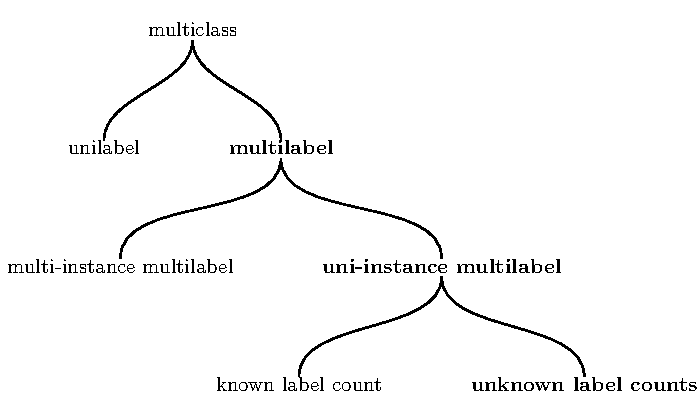
\includegraphics[width=.9\linewidth]{./tree/Tree.pdf}
% \caption{\label{fig:tree} SIMPUL (bold) within the \emph{multiclass}
% nomenclature
% \hvk{figure is not referenced in text, bold is unclear in figure}
% \daan{I think it should go. And if it stays: uni -> single.}
% % Clarifying ``multiclass'' classification problems. In this paper we focus on
% % the uni-instance, multilabel, multiclass classification problem with a
% % varying number of labels (the bottom right hand side of the tree).
% }
% \end{figure}% \mdr{Image source ...}

%%% Local Variables:
%%% mode: latex
%%% TeX-master: "../main"
%%% End: